\begin{frame}[t]{\dechorate: realization}

    \vspace{-2mm}
    \begin{block}{\dechorate: echo-aware dataset}
        \begin{description}
            \item<2->[Recorded:] Acoustic lab of Bar'Ilan (Shoebox)
            \item<3->[Annotated:] manually
            \item<4->[Collaboration:]  prof. Sharon Gannot and ing. Pinchas Tandeitnik
        \end{description}
    \end{block}

    \only<5>{
    \begin{block}{Key features:}
        \begin{itemize}
            \item revolving panels (different $\mathtt{RT}_{60}$ and echo prominency)
            \item 6 nULA with 5 mics and 4 sound sources
            \item geometry annotated \& echo annotated
            \item measured RIRs $\leftarrow$ (matching) $\rightarrow$ simulated RIRs
        \end{itemize}
    \end{block}
    }

    \vfill
    \only<1-4>{
        \begin{center}
            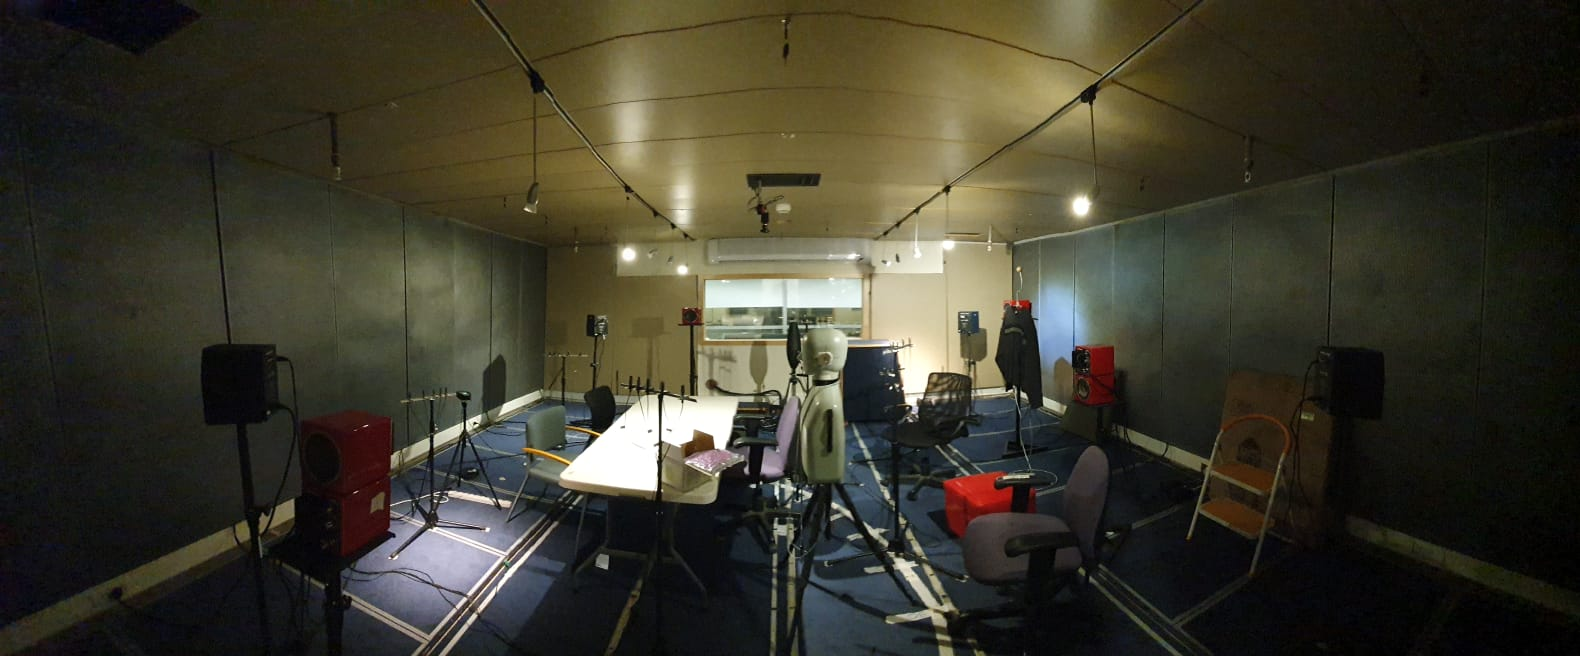
\includegraphics[trim={0 0 0 10em},clip,width=\textwidth]{figures/dechorate/fornitures.jpg}
        \end{center}
    }
    \only<5->{
        \begin{columns}[T,onlytextwidth]
            \begin{column}{0.3\textwidth}
                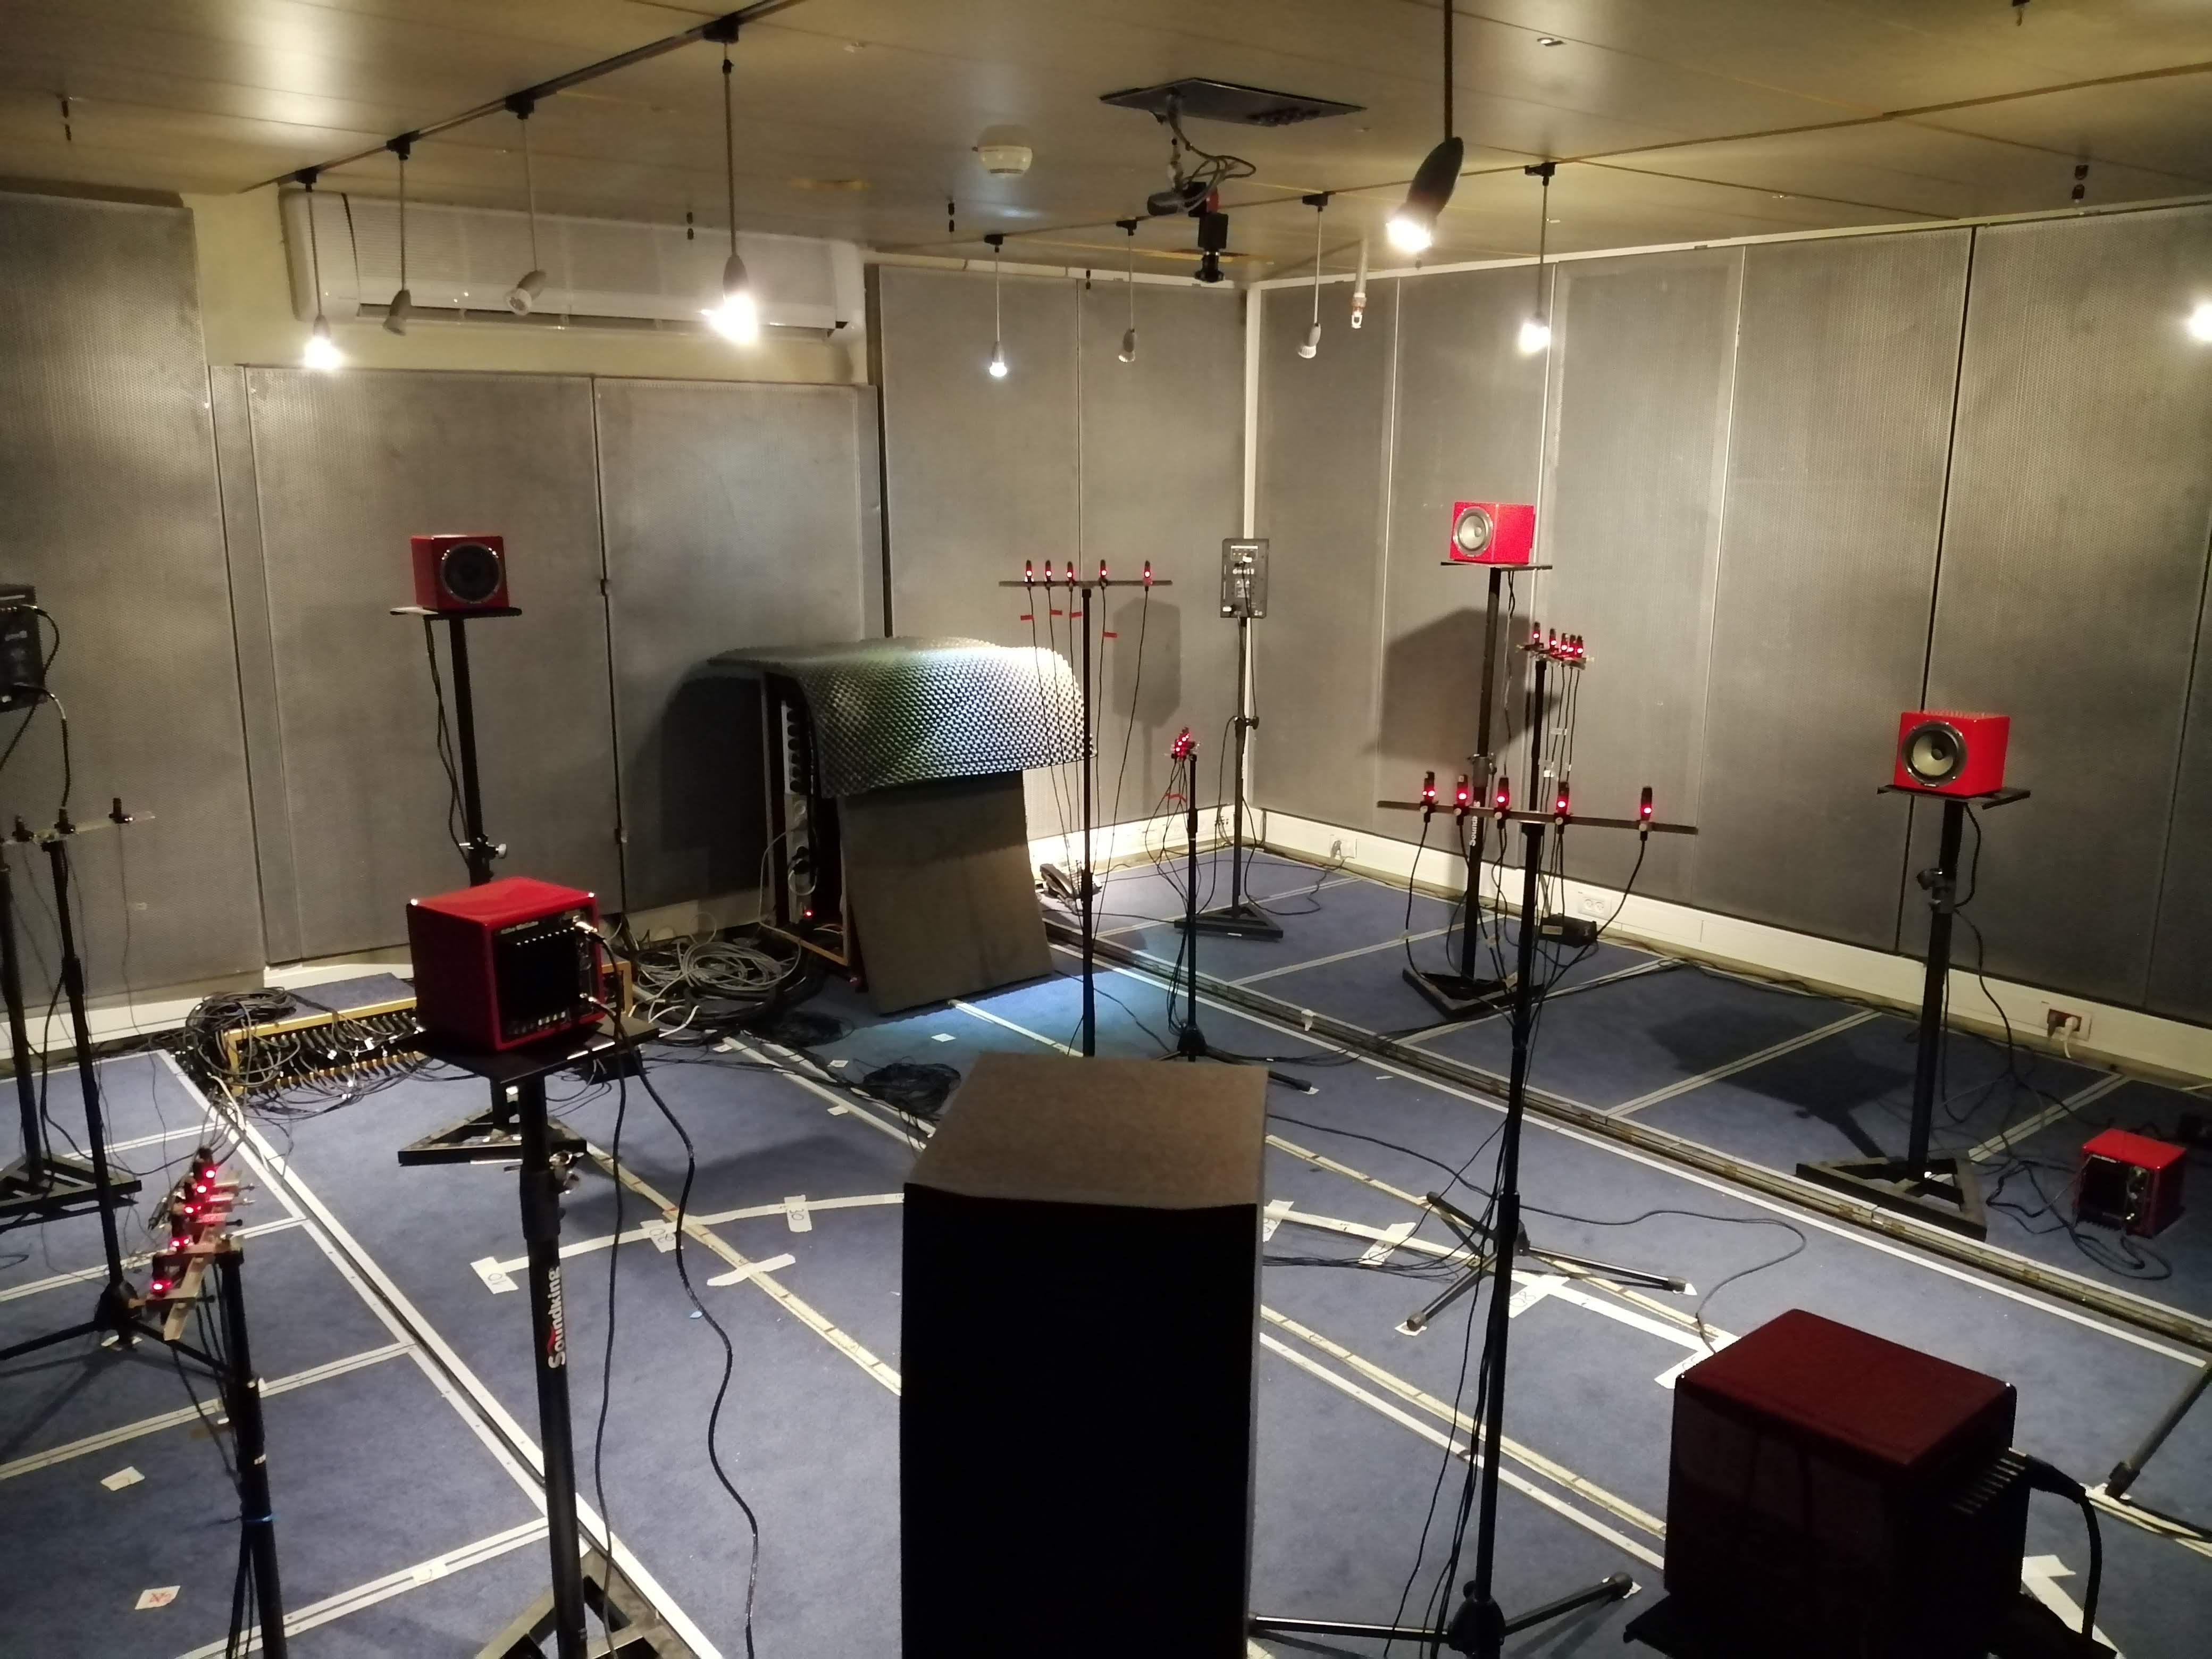
\includegraphics[width=\textwidth]{figures/dechorate/recording_setup}
            \end{column}\hfill
            \begin{column}{0.3\textwidth}
                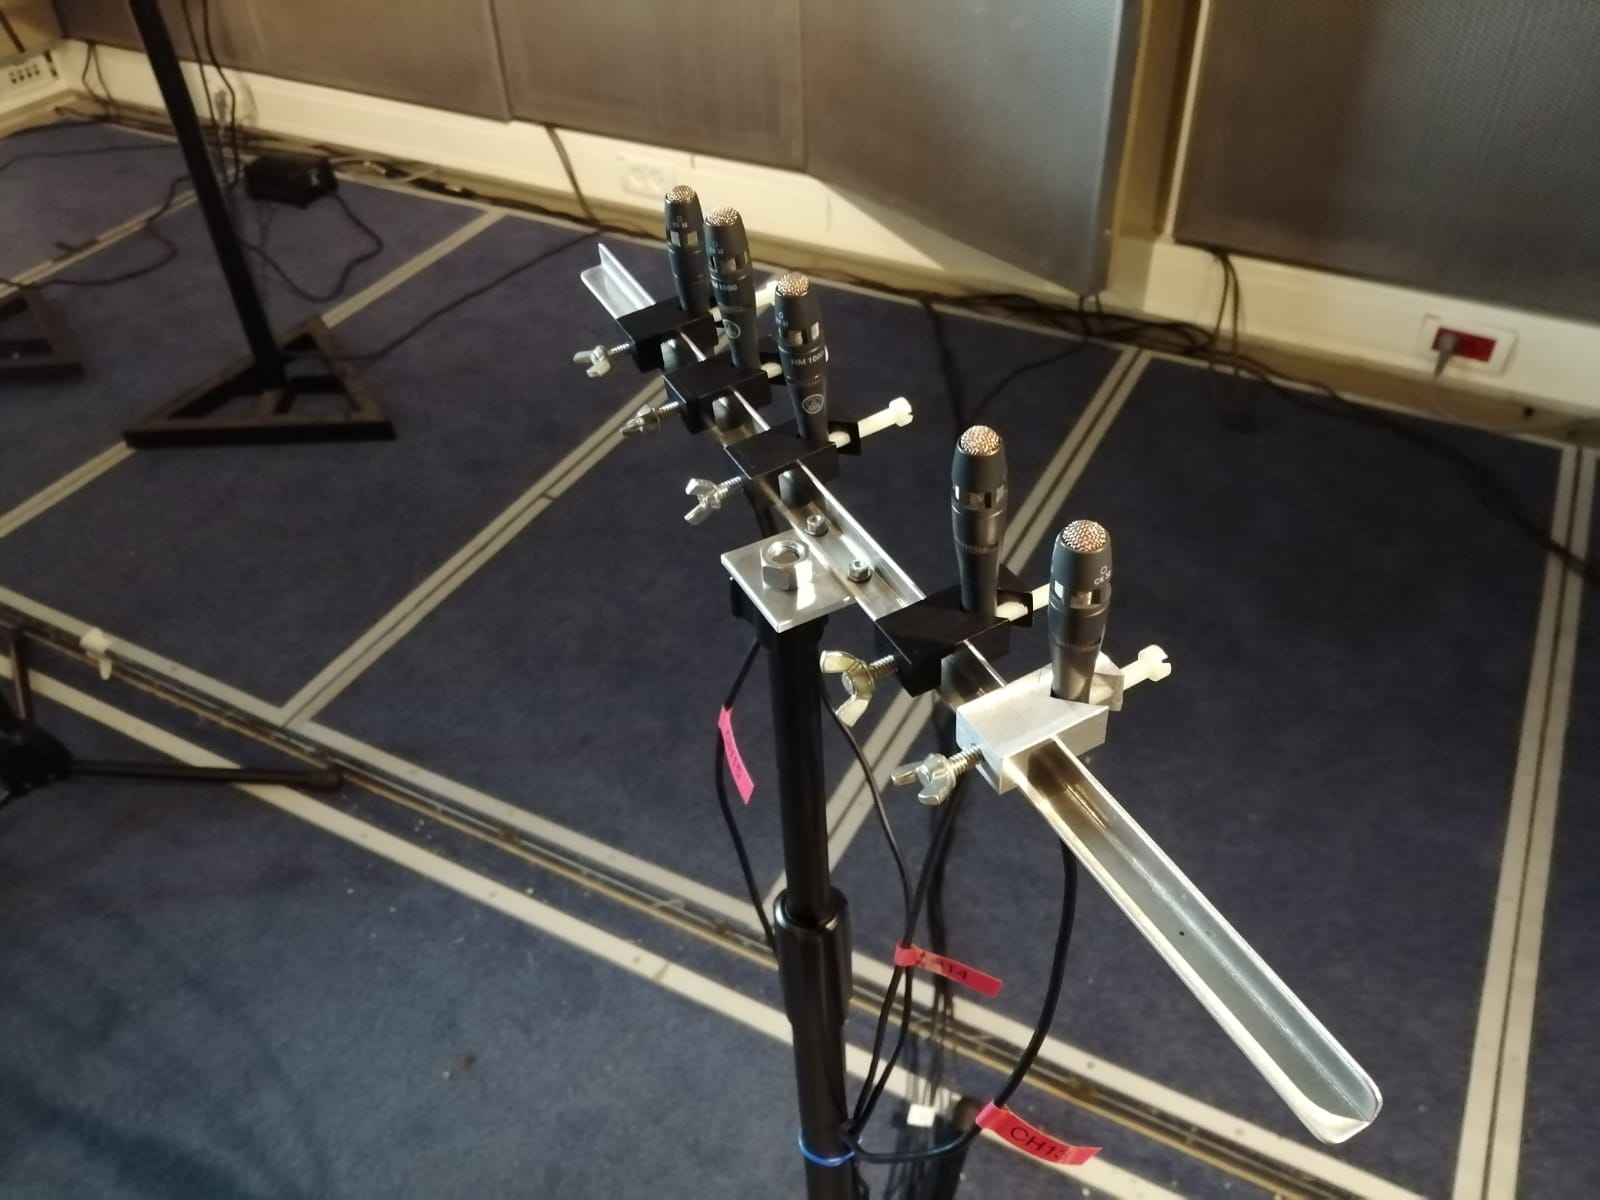
\includegraphics[width=\textwidth]{figures/dechorate/mic}
            \end{column}\hfill
            \begin{column}{0.3\textwidth}
                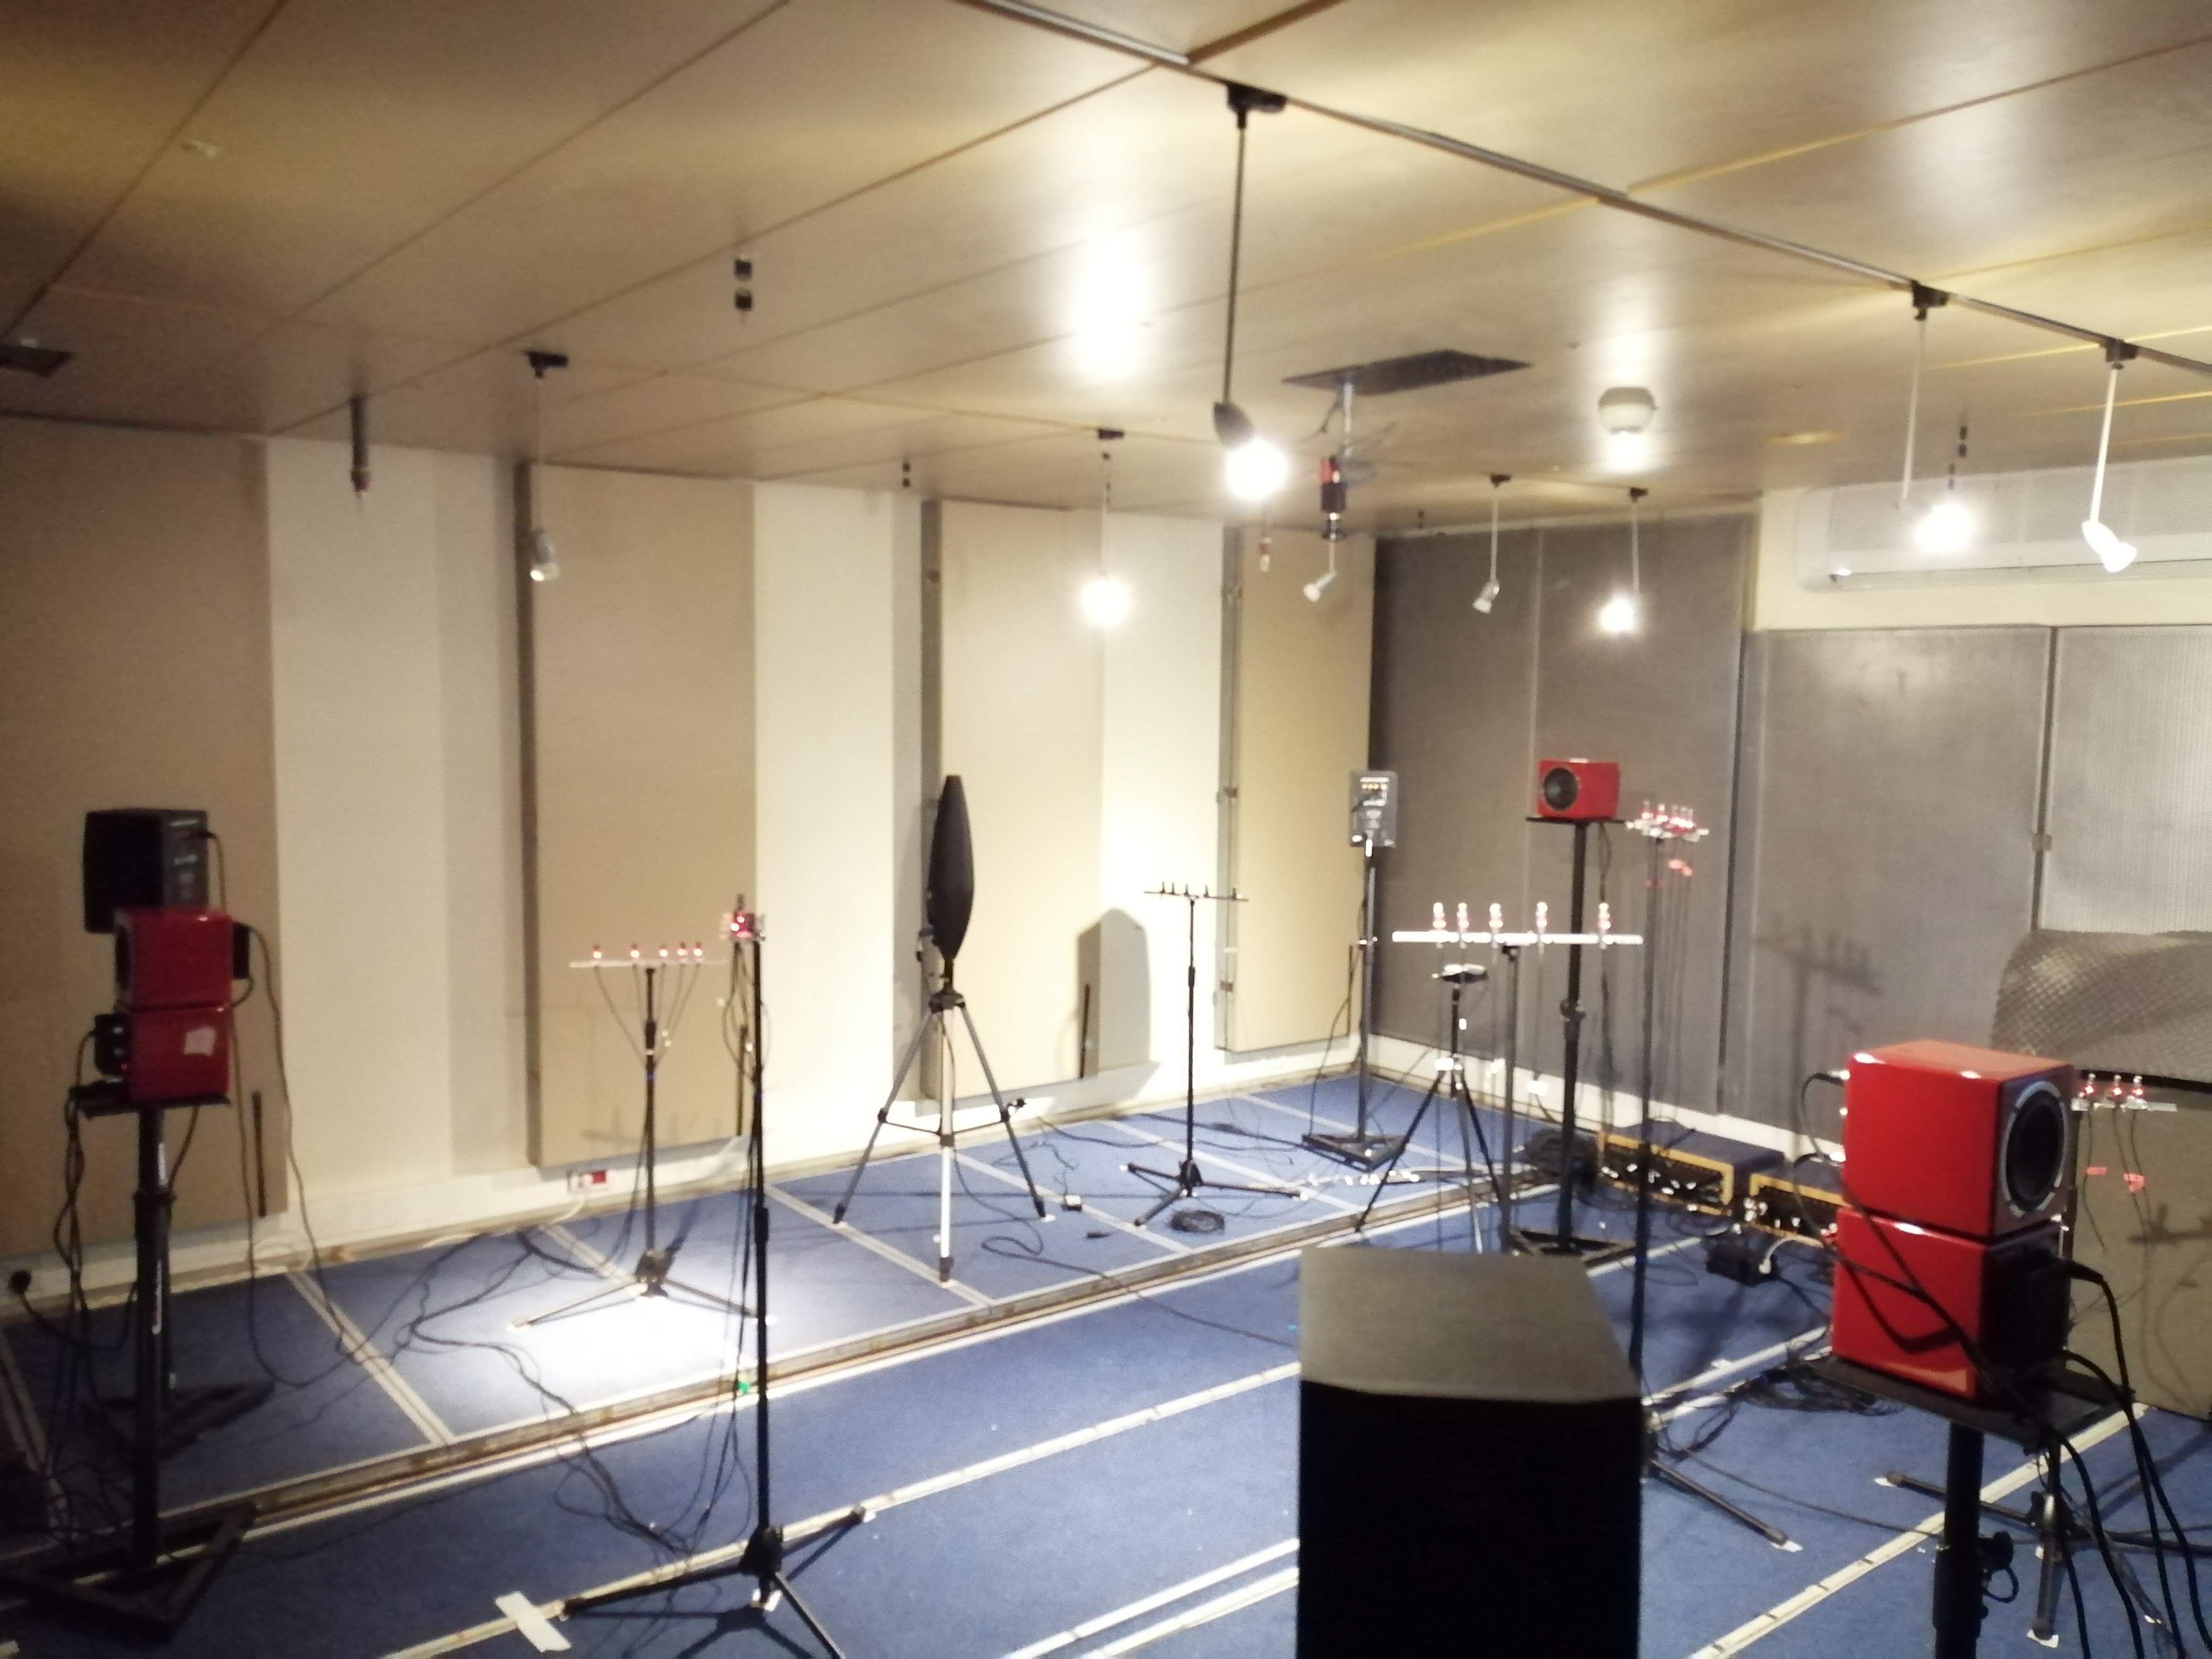
\includegraphics[width=\textwidth]{figures/dechorate/panels}
            \end{column}
        \end{columns}
    }

\end{frame}

\begin{frame}[t]{\dechorate: annotation}

    \begin{enumerate}
        \item<1-> \textbf{RIR estimation} with \textbf{chirps signal}~\cite{farina2007advancements,szoke2019building}
        \item<2-> \textbf{IPS calibration} with beacon $\longrightarrow$ mic and src positioning ($\pm 2$ cm)
        \item<3-> \textbf{GUI for annotation}
        \\\alert{Skyline}, \alert{Matched Filter}, Assisted Peak Picking
        \item<4-> Refined position with \textbf{Least Square optimization}
        \item<5-> \textbf{iterate including ceiling} (perfectly flat)
    \end{enumerate}

    \vfill
    \visible<3->{
        \begin{center}
            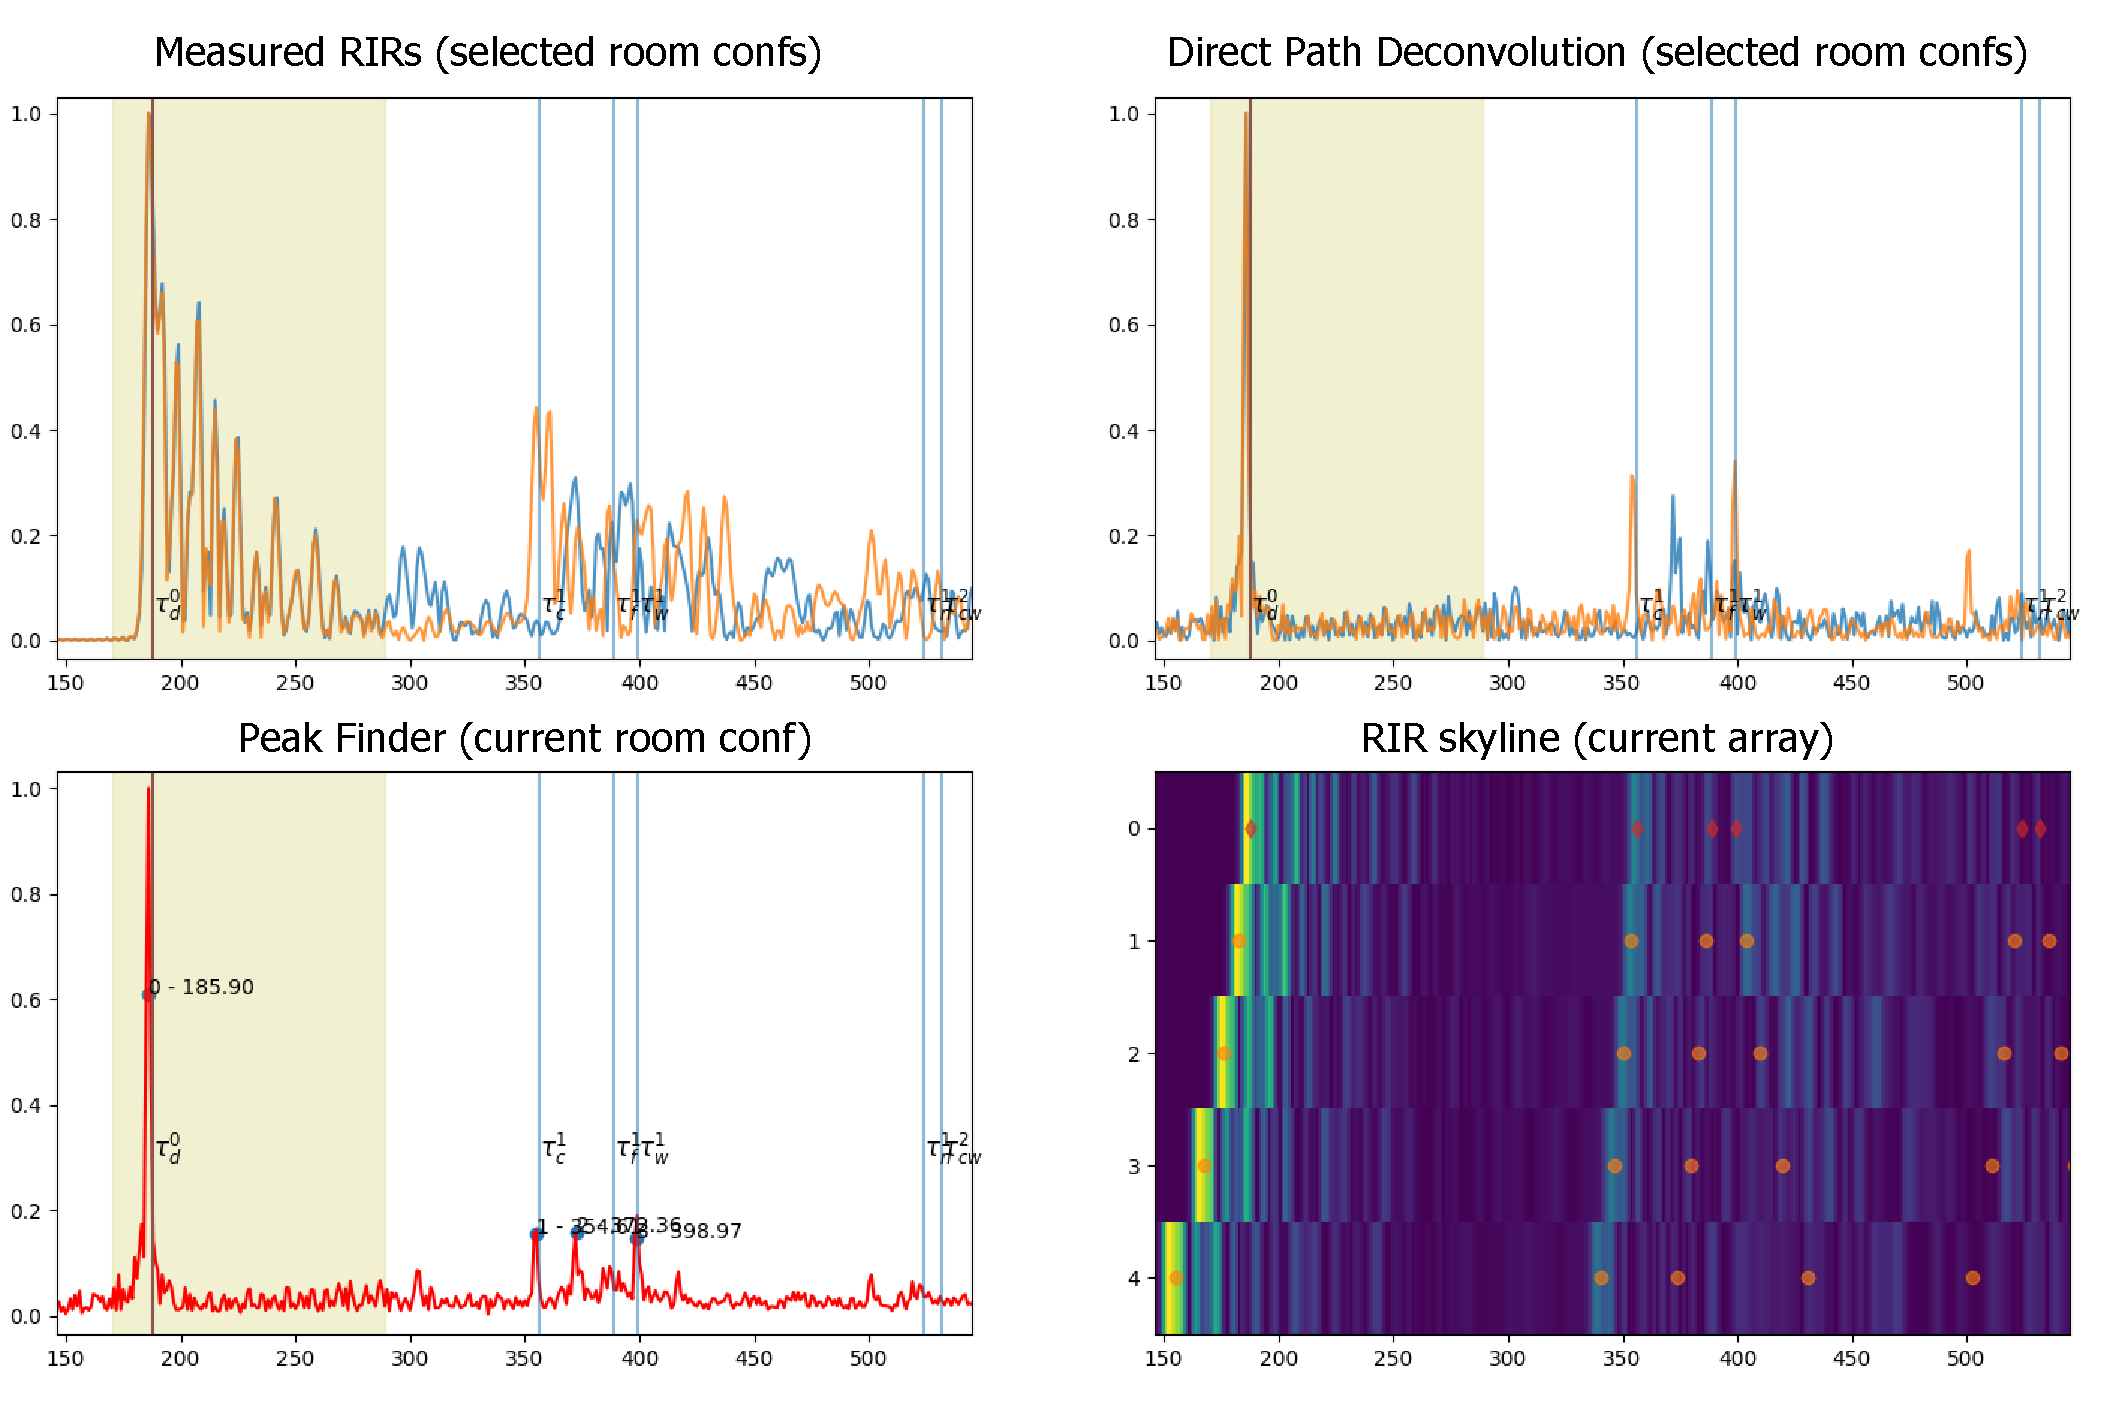
\includegraphics[width=.8\textwidth]{figures/dechorate/labeling_tool.pdf}
        \end{center}
    }

    % \vfill
    % \only<3>{
    %     \begin{adjustbox}{minipage=.8\textwidth,margin=0pt \smallskipamount,center}
    %         \centering
    %         \small
    %         \begin{tabular*}{\linewidth}{@{\extracolsep{\fill}}lllll@{}}
    %             \toprule
    %             & Metrics      & $\mathtt{bIPS}$  & $\mathtt{dMDS}$ & $\mathtt{dcMDS}$          \\
    %             \midrule
    %             \multicolumn{1}{c}{\multirow{2}{*}{\rotatebox{90}{\footnotesize Geom.}}}
    %             &   Max.             & 0            & $6.1$          & $1.07$        \\
    %             &   Avg.$\pm$Std.    & 0            & $1.8\pm1.4$    & $0.39\pm0.2$  \\
    %             % \rule{0pt}{0.1em}\\
    %             \midrule
    %             \multicolumn{1}{c}{\multirow{2}{*}{\rotatebox{90}{\footnotesize Signal}}}
    %             &   Max.          & $5.86$         & $1.20$         & $1.86$       \\
    %             &   Avg.$\pm$Std. & $1.85\pm 1.5$  & $0.16\pm0.2$   & $0.41\pm0.3$ \\
    %             % \rule{0pt}{0.1em}\\
    %             \midrule
    %             \multicolumn{1}{c}{\multirow{3}{*}{\rotatebox{90}{\footnotesize Mismatch}}}
    %             &  GoM (1.0 ms)   & $97.9 \%$      & $93.4 \%$      & $98.1 \%$ \\
    %             &  GoM (0.1 ms)   & $26.6 \%$      & $44.8 \%$      & $53.1 \%$ \\
    %             &  GoM (0.05 ms)  & $12.5 \%$      & $14.4 \%$      & $30.2 \%$ \\
    %             \bottomrule
    %         \end{tabular*}

    %         \vspace{3mm}
    %         \textcolor{gray}{GoM = Goodness of Match ($\neq$ error, because no groundtruth)}
    %     \end{adjustbox}
    % }

\end{frame}

\begin{frame}{\dechorate --- Annotation}
    \begin{center}
        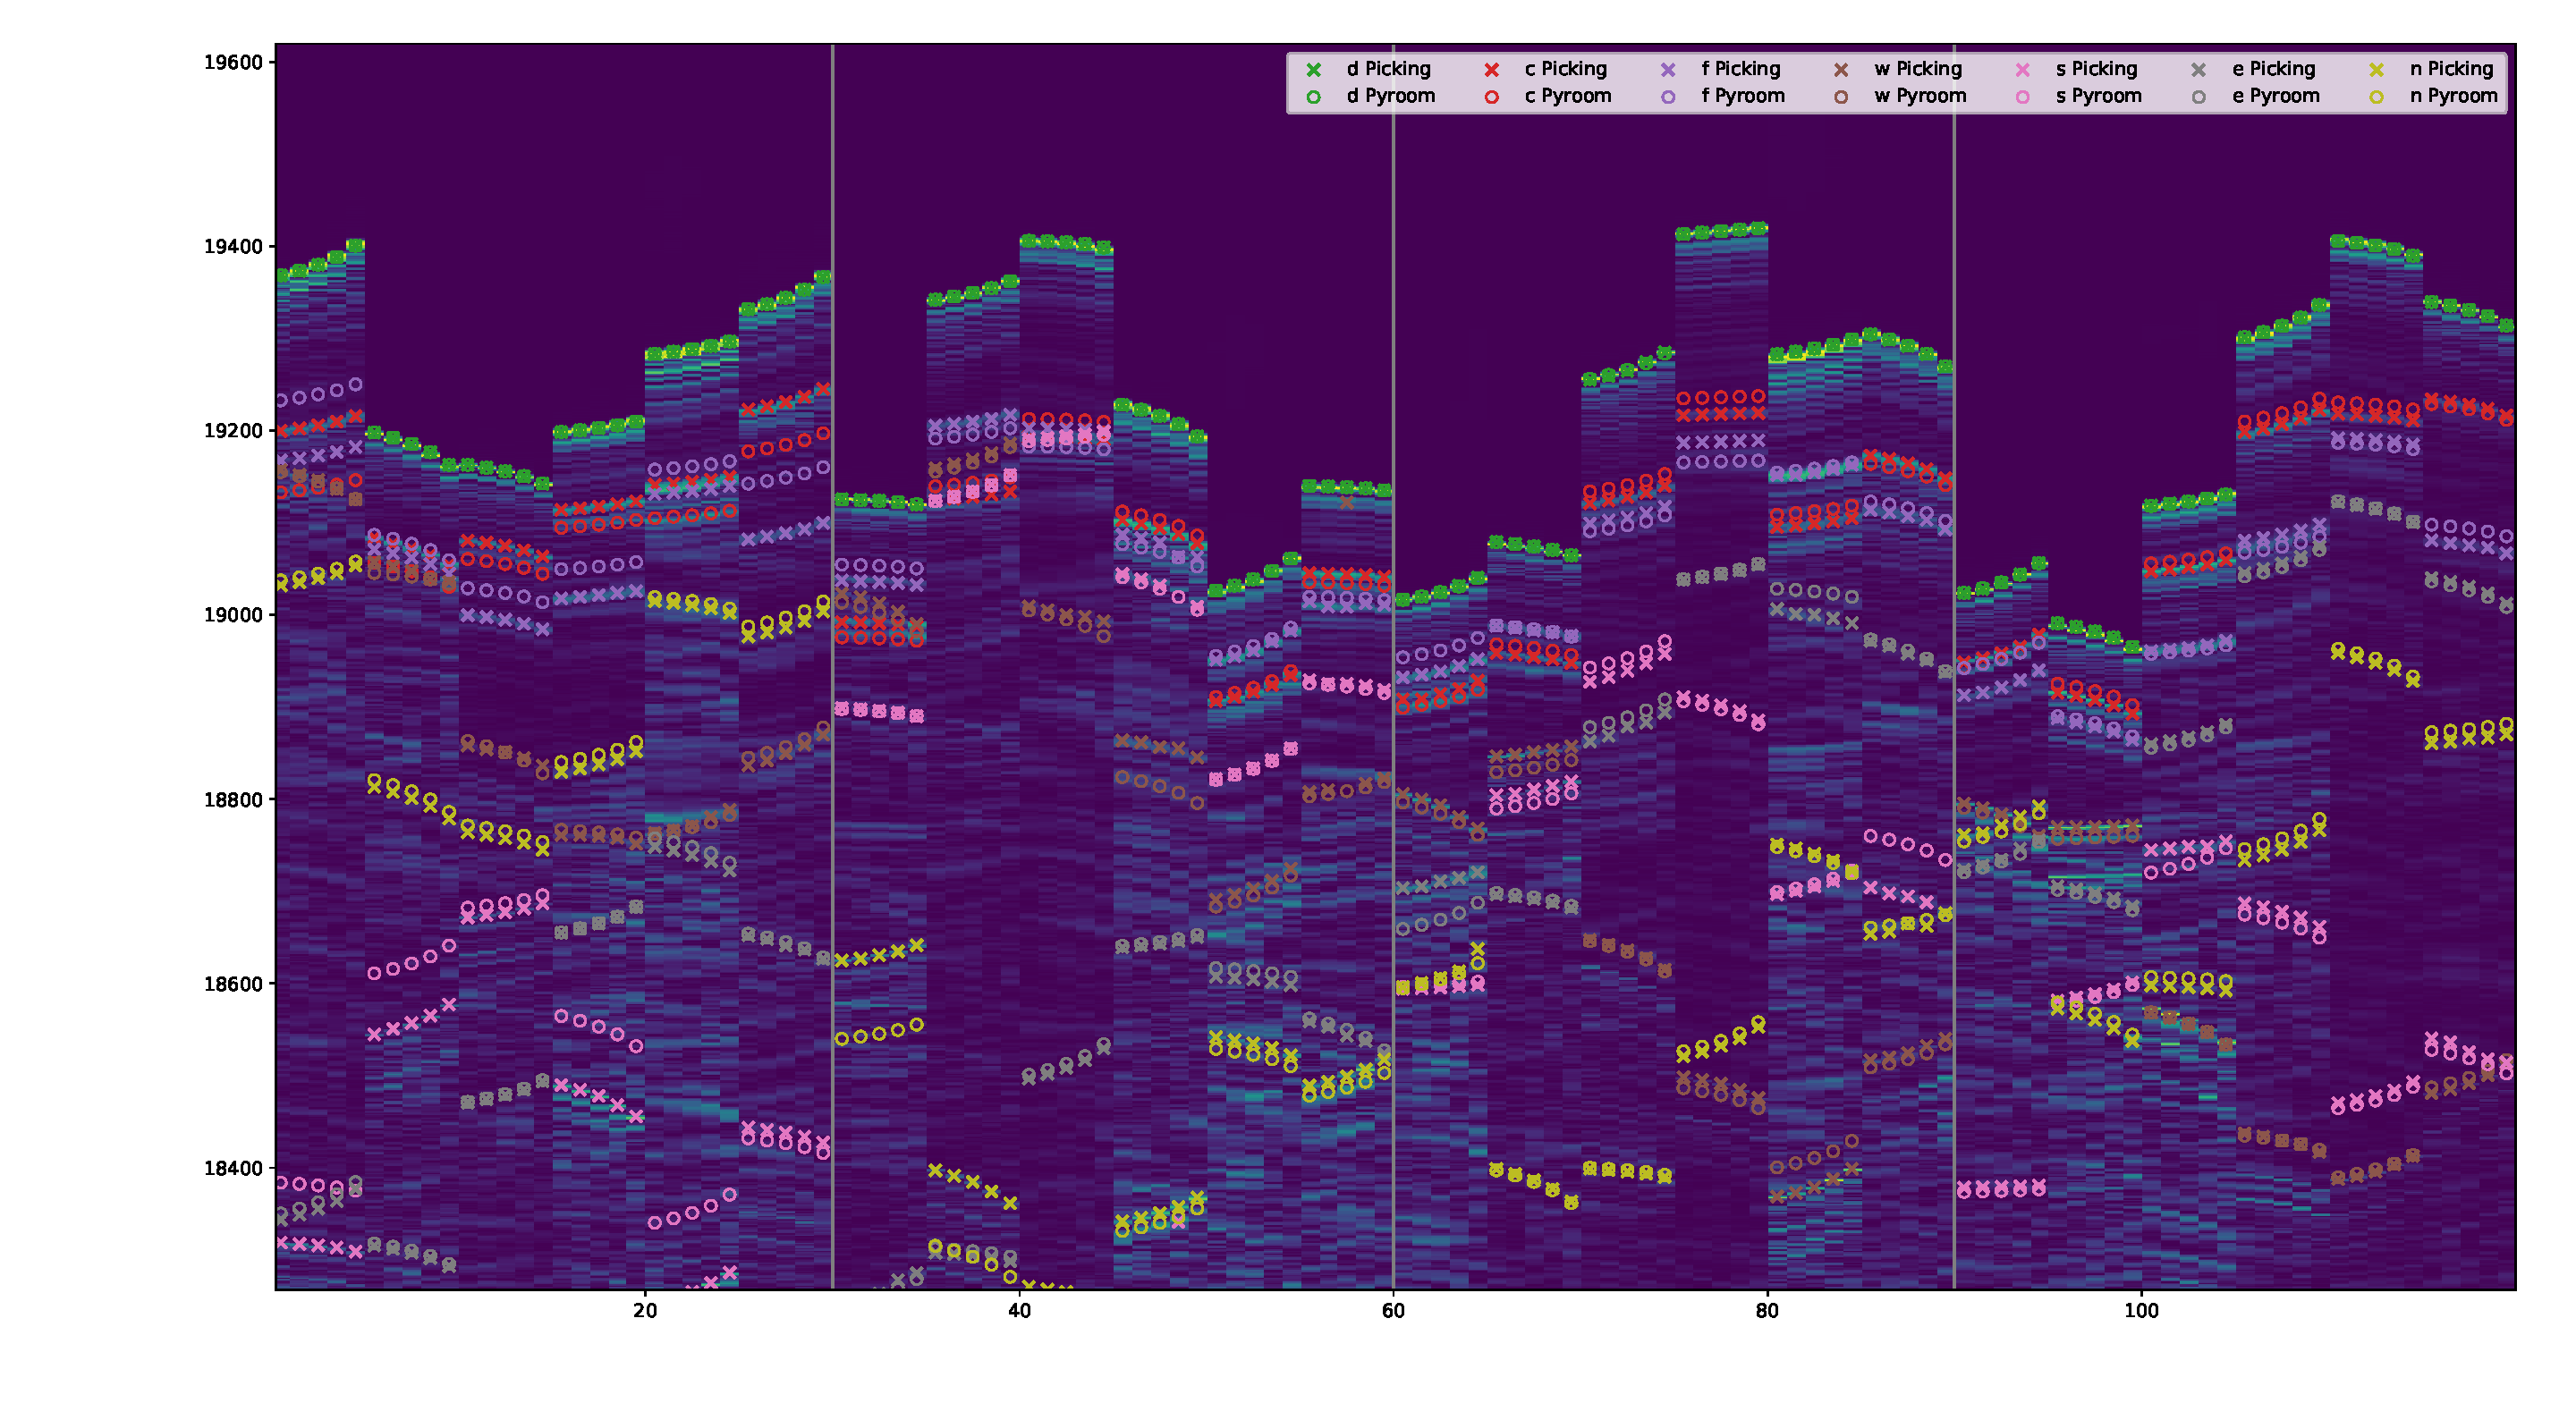
\includegraphics[trim={10em 0 0 0},clip,width=\linewidth]{figures/dechorate/rir_skyline_final_mod4paper.pdf}
    \end{center}

    \vspace*{-2mm}
    RIR Skyline showing
    \begin{itemize}
        \item absolute value of stacked RIRs as a figure
        \item[$\times$] manual echo annotation
        \item[$\circ$] \textit{matching} echo annotation for \texttt{ISM simulator}
    \end{itemize}
\end{frame}


\begin{frame}[t]{Room Geometry Estimation (RooGE) with \dechorate}

    \begin{mydefblock}{Room Geometry Estimation (RooGE)}
        Estimate shape, volume or reflector position from signal (or form TOAs).
    \end{mydefblock}

    \pause
    If TOAs annotation (label and value) is available $\implies$ \alert{Image Source Inversion}
    \\For each wall/label:
    \begin{enumerate}
        \item<3-> TOA $\kto$ image source position via 3D multilateration
        \item<4-> image source position $\kto$ reflector estimation via geometric reasoning
    \end{enumerate}
    \visible<4->{
        \centering
        \footnotesize\textcolor{gray}{other methods differ for priors and setup~\cite{filos2011robust,antonacci2012inference,crocco2017uncalibrated}}
    }


    \begin{columns}
        \begin{column}{.48\textwidth}
            \includegraphics<3-4>[width=\textwidth]{figures/dechorate/estimated_image}
        \end{column}\hfill
        \begin{column}{.48\textwidth}
            \includegraphics<4>[width=\textwidth]{figures/dechorate/estimated_reflector}
        \end{column}
    \end{columns}

    \only<5>{
        \begin{adjustbox}{minipage=.9\textwidth,margin=0pt \smallskipamount,center}
            \centering
            \small
            \begin{tabular*}{\linewidth}{c|cc|cc|cc|cc}
                \toprule
                source id &	1	& &	2	& &	3	& &	4 &	\\
                wall &	DE&	AE&	DE&	AE&	DE&	AE&	DE&	AE\\
                \hline
                west &	0.74	& $\ang{8.99}$      & 4.59	& $\ang{8.32}$  & 5.89	& $\ang{5.75}$	& $\mathbf{0.05}$    & $\mathbf{\ang{2.40}}$\\
                east &	$\mathbf{0.81}$	& $\mathbf{\ang{0.08}}$      & 0.9	& $\ang{0.50}$	&$\mathit{69.51}$	& $\mathit{55.70}^\circ$	& 0.31    & $\ang{0.21}$\\
                south&	3.94	&$\mathit{16.08}^\circ$      & $\mathbf{0.18}$	& $\ang{1.77}$	&$\mathit{14.37}$ & $\mathit{18.55}^\circ$	& 0.82    & $\mathbf{\ang{1.65}}$\\
                north&	1.34	& $\ang{0.76}$	    & 1.40	& $\ang{8.94}$	& $\mathbf{0.63}$	& $\mathbf{\ang{0.17}}$	& 2.08    & $\ang{1.38}$\\
                floor&	$\mathbf{5.19}$	& $\mathbf{\ang{1.76}}$	    & 7.27	& $\ang{2.66}$	& 7.11	& $\ang{2.02}$	& 5.22    & $\ang{1.90}$\\
                ceiling&1.16	& $\ang{0.28}$	    & 0.67	& $\ang{0.76}$	& $\mathbf{0.24}$	& $\ang{1.16}$	& $0.48$    & $\mathbf{\ang{0.26}}$\\
                \bottomrule
                \end{tabular*}
        \end{adjustbox}
        \begin{center}
            \small
            \textcolor{gray}{Distance Error (DE) [cm] and Angular Error (AE), \textbf{best}, \textit{outliers}}
        \end{center}

    }

\end{frame}